%\documentclass[11pt,a4paper,uplatex,dvipdfmx]{ujarticle} 		% for uplatex
\documentclass[11pt,a4j,dvipdfmx]{jarticle} 					% for platex
\input{pieces/form00_header} % pieces
\input{pieces/kakenhi7} % pieces
\input{pieces/form01_header} % pieces
% ===== Global year-dependent definitions for the Kakenhi form ===========
%　基本情報
\newcommand{\研究開始年度}{2027}
\newcommand{\研究開始元号年度}{09}	%令和

\newcommand{\一年目西暦}{2027}
\newcommand{\二年目西暦}{2028}
\newcommand{\三年目西暦}{2029}
\newcommand{\四年目西暦}{2030}
\newcommand{\五年目西暦}{2031}
\newcommand{\六年目西暦}{2032}

\newcommand{\一年目}{9}
\newcommand{\二年目}{10}
\newcommand{\三年目}{11}
\newcommand{\四年目}{12}
\newcommand{\五年目}{13}
\newcommand{\六年目}{14}

\newcommand{\一年目J}{９}
\newcommand{\二年目J}{１０}
\newcommand{\三年目J}{１１}
\newcommand{\四年目J}{１２}
\newcommand{\五年目J}{１３}
\newcommand{\六年目J}{１４}


 % pieces
\input{pieces/hook3} % pieces
%#Name: kiban_s
\input{pieces/form04_jsps_headers} % pieces
\input{pieces/form04_kiban_s_header} % pieces
% ===== Global definitions for the Kakenhi form ======================
%　基本情報
%
%------ 研究課題名  -------------------------------------------
\newcommand{\研究課題名}{加速器実験による短距離バリオン間相互作用の解明と中性子星ハイペロンパズルの解決}

%----- 研究機関名と研究代表者の氏名-----------------------
\newcommand{\研究機関名}{東北大学}
\newcommand{\研究代表者氏名}{市川裕大}
\newcommand{\me}{\underline{\underline{Y.~Ichikawa}}}
%---- 研究期間の最終年度 ----------------
\newcommand{\研究期間の最終元号年度}{13}  %令和で、半角数字のみ
%========================================

\input{pieces/inst_general_images} % pieces
%inst_kiban_s.tex
\newcommand{\EnvironmentInstructions}{%
	\textcolor{red}{(\texttt{\textbackslash EnvironmentInstructions}をコメントアウトしてください。)}\\
	\includegraphicsFullWidth{subject_headers/inst_env.pdf}
}
 % pieces
% user07_header
% ===== my favorite packages ====================================
% ここに、自分の使いたいパッケージを宣言して下さい。
\usepackage{wrapfig}
\usepackage{capt-of}
%\usepackage{amssymb}
%\usepackage{mb}
%\DeclareGraphicsRule{.tif}{png}{.png}{`convert #1 `dirname #1`/`basename #1 .tif`.png}
\usepackage{lineno}

% ===== my personal definitions ==================================
% ここに、自分のよく使う記号などを定義して下さい。
\newcommand{\klpionn}{K_L \to \pi^0 \nu \overline{\nu}}
\newcommand{\kppipnn}{K^+ \to \pi^+ \nu \overline{\nu}}

% ----- 業績リスト用 -------------
\newcommand{\paper}[6]{%
	% paper{title}{authors}{journal}{vol}{pages}{year}
	\item ``#1'', #2, #3 {\bf #4}, #5 (#6).			% お好みに合わせて変えてください。
}

\newcommand{\etal}{\textit{et al.\ }}
\newcommand{\ca}[1]{*#1}	% corresponding author;   \ca{\yukawa}  みたいにして使う
\newcommand{\invitedtalk}{招待講演}

\newcommand{\yukawa}{H.~Yukawa}					% no underline
%\newcommand{\yukawa}{\underline{\underline{H.~Yukawa}}}	% with 2 underlines
\newcommand{\tomonaga}{S.~Tomonaga}

\newcommand{\prl}{Phys.\ Rev.\ Lett.\ }		% よく使う雑誌も定義すると楽

% ===== 欄外メモ ==================
\newcommand{\memo}[1]{\marginpar{#1}}
%\renewcommand{\memo}[1]{}	% 全てのメモを表示させないようにするには、行頭の"%"を消す

\input{pieces/hook5} % pieces

\begin{document}
\input{pieces/hook7} % pieces
%#Split: 01_purpose_plan  
%#PieceName: p01_purpose_plan
\input{pieces/p01_purpose_plan_00}
\section{研究目的、研究方法など}
%　　　　＜＜最大　6ページ＞＞

%s02_purpose_plan_with_abstract
% \JSPSInstructions		% <-- 留意事項。これは消すか、コメントアウトしてください。
\noindent
\textbf{（概要）}\\
%begin 研究目的及び研究計画の概要空行付き ＝＝＝＝＝＝＝＝＝＝＝＝＝＝＝＝＝＝＝＝
	本研究の目的は、高密度天体である中性子星の内部構造を決定づける「ハイペロン・パズル」の解決に向け、ハドロン加速器実験を用いた新手法により、ハイペロン（$\Lambda$粒子）と核子の間に働く短距離相互作用を解明することである。
	
	理論的には、$\Lambda N$間の引力は$2\pi$中間子交換（中間状態としての$\Sigma$粒子）が担うと考えられているが、高密度媒質中では核子のパウリ排他律によりこの過程が抑制され、結果として強い斥力が現れることが示唆されている。本研究では、(1) $\Sigma N$カスプ分光（E90）による$2\pi$交換寄与の定量化、(2) $pA$フェムトスコピー（E88）による媒質中の短距離力測定、(3) $\Lambda p$散乱実験（HYPS）による真空中の短距離力測定、という3つの独創的実験データを、カイラル摂動論に基づき統合的に解析することで、高密度での斥力芯シナリオの正否に決着をつける。
	
	\vspace*{7zw}	% （概要）と（本文）の間が10行程度になるよう、必要に応じて値を調整してください。	
%end 研究目的及び研究計画の概要空行付き ＝＝＝＝＝＝＝＝＝＝＝＝＝＝＝＝＝＝＝＝

\noindent
\rule{\linewidth}{1pt}\\
\noindent
\textbf{（本文）}
%begin 研究目的と研究計画	 ＝＝＝＝＝＝＝＝＝＝＝＝＝＝＝＝＝＝＝＝

\subsection{研究課題の核心をなす学術的「問い」と着想に至った経緯}
私たちの宇宙には、通常の物質密度の数倍に達する極限状態が実現している天体が存在する。それが「中性子星」である。中性子星の中心部では、原子核密度の数倍（数億トン/cm$^3$）という、地上の実験室では再現不可能な超高密度物質が形成されている。この極限環境において、物質がどのような形態をとり、どのような相互作用によって巨大な重力を支えているのかを解明することは、現代核物理学・天体物理学における最重要課題の一つである。

通常の原子核は、アップ（$u$）クォークとダウン（$d$）クォークからなる陽子と中性子（核子）によって構成されている。しかし、自然界にはこれらこれらとは別に、第三のクォークである「ストレンジ（$s$）」クォークを含むバリオン（重粒子）が存在し、これらを総称して「ハイペロン」と呼ぶ。その中でも最も軽いものが$\Lambda$（ラムダ）粒子である。$\Lambda$粒子は、陽子・中性子と同様の強相互作用（ハドロンを束ねる力）を経験する粒子でありながら、ストレンジクォークという通常の核子にはない成分を含んでいる。

\subsubsection{ハイペロン・パズル：理論と天体観測の深刻な矛盾}
これまでのハイパー核物理学の研究により、$\Lambda$粒子が原子核と結合した「$\Lambda$ハイパー核」が数多く発見されている。これらの束縛エネルギーの系統的な研究から、標準原子核密度（$\rho_0$）において$\Lambda$粒子が感じるポテンシャルの深さは約 $-30$~MeV であることが確定している。これは、核子が感じる約 $-50$~MeV に比べれば浅いものの、原子核中において$\Lambda$粒子が明確な「引力」を感じていることを示す決定的な実験事実である。

この「引力」の存在は、中性子星の物理において深刻な矛盾を引き起こす。中性子星の中心部に向かって密度が高まると、核子のフェルミエネルギーが増大する。ある閾値を超えると、中性子をさらに詰め込むよりも、引力的なポテンシャルを感じる$\Lambda$粒子を生成したほうが系のエネルギーが低くなるため、中性子星内部でのハイペロン出現は物理的な必然となる。しかし、核物理学の標準的な理論モデルに基づく状態方程式（Equation of State; EoS）の予測によれば、ハイペロンの出現はEoSを劇的に軟化（圧力を低下）させ、観測されている2太陽質量（$2M_\odot$）もの重い中性子星を支えることができなくなる。これが「ハイペロン・パズル」である。

本研究が挑む核心的な問いは、\textbf{「標準密度で引力的であるはずの$\Lambda$粒子が、なぜ中性子星深部の超高密度下ではその出現が抑制（あるいはその影響が排除）され、結果として重い中性子星を支えることが可能になっているのか」}という点にある。理論的には、$\Lambda$粒子が出現すれば状態方程式は劇的に軟化し、観測されている2倍の太陽質量を持つ中性子星を支えることは不可能になる。したがって、超高密度下において$\Lambda$粒子の出現をエネルギー的に禁止する、あるいは出現してもなお強い圧力を維持させる「未知の斥力メカニズム」を実験的に立証することこそが、ハイペロン・パズル解決の鍵となる。

\subsubsection{本研究の着想に至った経緯：媒質中での相互作用変化への着目}
\begin{wrapfigure}{r}{2.2cm}
  \centering
  
\includegraphics[width=2.0cm]{figs/2piExchange.png}
  \caption{$\Lambda N$間の$2\pi$交換。}
  \label{fig:2pi}
\end{wrapfigure}
$\Lambda N$間の引力は、ミクロには$\Lambda$が中間状態で$\Sigma$粒子へと遷移しながら2つの$\pi$中間子を交換する「$2\pi$交換プロセス」（図\ref{fig:2pi}）が担っていると考えられている。申請者は、この引力プロセスが媒質（高密度物質）中に入ると、量子力学的なパウリ排他律によって強く抑制（パウリ・ブロッキング）される点に着目した。
もし、高密度下で引力が消失し、代わりにクォークの重なりに起因する斥力が支配的になるならば、ハイペロンの出現は抑制される、あるいは出現しても重い星を支える硬いEoSが維持される。この「媒質中でのダイナミックな相互作用変化」を多角的な実験データから切り出すことが、本研究の独創的な着想である。

\subsection{本研究の目的及び研究計画・方法}
\subsubsection{研究の目的：高密度バリオン間相互作用の完全確定}
本研究の目的は、真空中および高密度媒質中における$\Lambda N$短距離相互作用を実験的に確定し、中性子星の状態方程式を決定づける斥力芯の起源に最終的な決着をつけることである。中性子星深部のような極限環境では、バリオン同士が重なり合う短距離での振る舞いが物理を支配する。本研究では、J-PARC加速器を用いた3つの異なるアプローチにより、引力と斥力の競合を定量的に分離し、ハイペロン出現を抑制する斥力メカニズムを実証する。

\subsubsection{研究計画・方法：本研究で何をどのように、どこまで明らかにしようとするのか}
本目的を達成するため、J-PARCハドロン実験施設のK1.8ビームラインを拠点とし、5カ年計画で以下の3つの独創的実験と理論統合を遂行する。

\begin{description}
    \item[1. $pA$フェムトスコピー（J-PARC E88）：高密度効果の直接抽出]\mbox{}\\
    これまで$\Lambda N$相互作用は主にハイパー核の結合エネルギーから研究されてきた。しかし図\ref{fig:femto_pot}に示す通り、$^{5}_{\Lambda}\mathrm{He}$等の束縛エネルギーを再現するだけでは、近距離でのポテンシャルの振る舞い（斥力芯の強さ）に多様なモデルを許容してしまい、一意に決定できないという「ハイパー核の限界」があった。
    
    この打破に向け、本研究では「フェムトスコピー」を導入する。これは、放出された2粒子の運動量相関を測定し、放出源の時空スケールや相互作用を探る手法である。特に、J-PARCの$pA$反応で生成される$R \sim 1$~fmの極小放出源を利用すると、相関関数$C(q)$はポテンシャルの短距離成分に極めて敏感になる。
    
    \begin{center}
      \begin{minipage}[t]{0.48\textwidth}
        \centering
        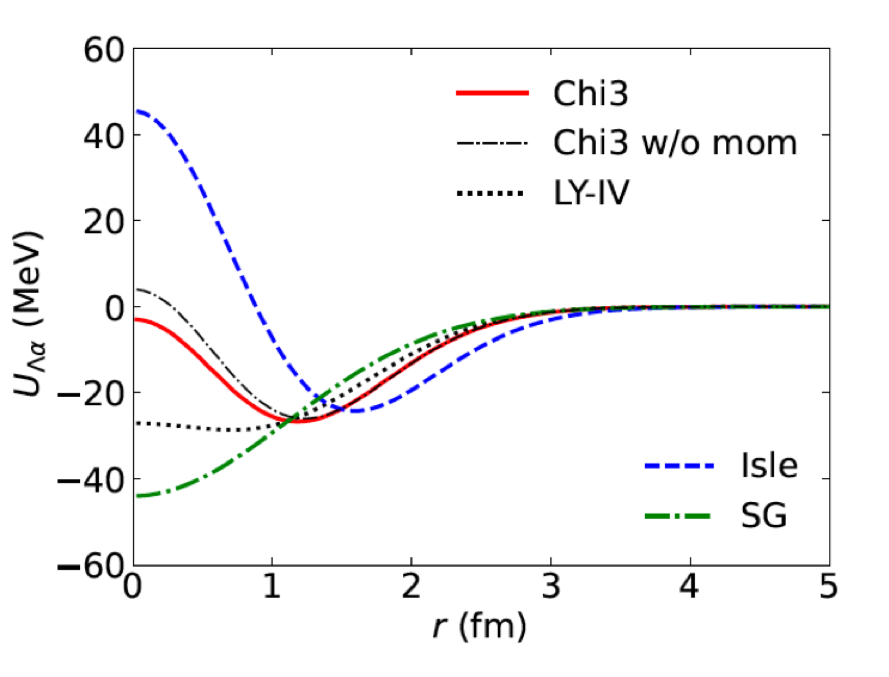
\includegraphics[width=\textwidth]{figs/femto_img_1.png}
        \captionof{figure}{モデル間で異なるポテンシャル。}
        \label{fig:femto_pot}
      \end{minipage}
      \hfill
      \begin{minipage}[t]{0.48\textwidth}
        \centering
        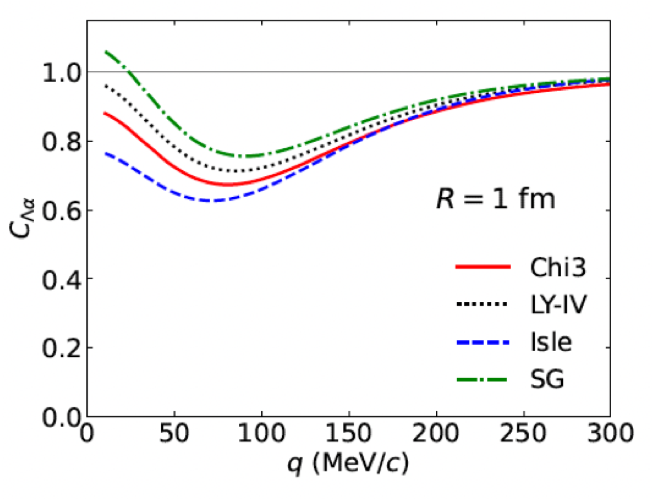
\includegraphics[width=\textwidth]{figs/femto_img_3.png}
        \captionof{figure}{相関関数によるモデルの分別。}
        \label{fig:femto_corr}
      \end{minipage}
    \end{center}
    
    図\ref{fig:femto_corr}に示す通り、$R=1$~fmの小ソース条件下では、異なる理論モデルが予測する相関関数に顕著な差異が現れる。本実験では、通常の原子核の2倍の密度を持つ$\alpha$粒子と$\Lambda$粒子の相関を測定し、高密度斥力芯シナリオの物理的実体を世界で初めて実験的に証明する。
    
    \item[2. $\Sigma N$カスプ分光（J-PARC E90）：チャンネル結合力の定量決定]\mbox{}\\
    \begin{minipage}[t]{0.50\textwidth}
      $d(K^-, \pi^-)\Lambda p n$ 反応スペクトルの$\Sigma N$生成閾値直下に現れる「$\Sigma N$カスプ」構造を精密観測する。ここで重要な物理パラメータが、低エネルギー散乱を特徴づける\textbf{「散乱長 ($a + ib$)」}である。散乱長とは、極低エネルギーの粒子から見た「相互作用の有効的な大きさ」を指し、実部 $a$ は散乱位相の変化（引力の強さ）を、虚部 $b$ は異なる粒子間への遷移（結合）の強さを表す。
    \end{minipage}
    \hfill
    \begin{minipage}[t]{0.45\textwidth}
      \vspace*{0pt}
      \centering
      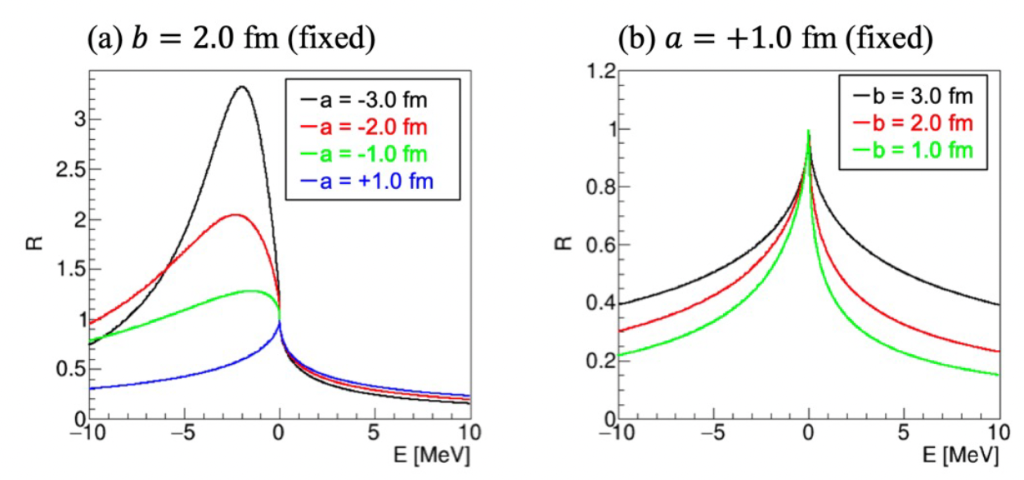
\includegraphics[width=\textwidth]{figs/e90_fig_scattering.png}
      \captionof{figure}{散乱長に対するカスプ形状の感度。}
      \label{fig:cusp}
    \end{minipage}
    
    図\ref{fig:cusp}に示すように、カスプ形状は $a, b$ の値に対し極めて敏感である。本実験では、世界最高分解能（$0.4$~MeV）でこの形状を捉え、散乱長の虚部から引力の源泉であるチャンネル結合強度を世界で初めて実験的に定量化する。
    \item[3. 真空中散乱実験（HYPS/E86）：裸の斥力芯サイズの直接測定]\mbox{}\\
    高強度の二次 $\Lambda$ ビームを用いた真空中散乱実験を実施する。斥力芯の情報が詰まった高運動量領域（高角散乱）のデータを大量取得することで、バリオン間の「裸の斥力芯半径」を $0.1$~fm 精度で確定させる。これは、媒質効果を正しく評価するための不動のリファレンスとなる。
\end{description}

これらの実験データを、研究分担者が推進するカイラル有効理論（ChPT）に基づく最新の計算に取り込む。ChPTにおける低エネルギー定数をこれらのデータにフィッティングさせ、核密度の数倍に至るまでの「密度依存性を持つ統一的相互作用モデル」を完成させる。これにより、中性子星の最大質量が $2M_\odot$ を超えることを示し、パズル解決の決定打を放つ。

\subsection{本研究の学術的独自性と創造性}
\subsubsection{独自性：相補的な3実験による多角的な検証}
本研究の独自性は、相互作用を「引力（結合力）・媒質（高密度）・斥力（短距離）」の3方向から同時に攻める点にある。これまで個別の実験では「引力と斥力の打ち消し合い」を分離できず、モデルに大きな不定性が残っていた。本研究では、それぞれの要素に特化した独立な実験データを組み合わせることで、この縮退を打破し、物理的に一意な結論を導き出す。

\subsubsection{創造性：極小放出源による短距離力の「増幅」観測}
本研究の創造性は、高エネルギー物理学の「フェムトスコピー」とハドロン物理の「精密分光」を融合させ、放出源サイズを $1$~fm 以下に絞り込む点にある。放出源を極小化することで、ポテンシャルの長距離成分（引力）の寄与を相対的に減らし、短距離の「斥力芯」の効果だけを劇的に増幅させて観測することができる。この革新的なアプローチにより、従来のハイパー核分光では到達不可能な「物性の根源」にアクセスする。

\subsection{関連する国内外の研究動向と本研究の位置づけ}
\subsubsection{国際的な研究動向：フェムトスコピーの隆盛と課題}
現在、欧州CERNのALICE実験や米国のSTAR実験において、高エネルギー重イオン衝突で生成される多数の粒子の相関を用いた研究が世界的なブームとなっている。しかし、これらの実験は放出源サイズが大きく（$R > 3$~fm）、引力が支配的で斥力芯の情報が薄れる点、および高温・低密度の「プラズマ冷却過程」であるため、中性子星に必要な「低温・高密度」の媒質効果を直接評価できないという課題がある。

\subsubsection{本研究の位置づけ：密度フロンティアと斥力芯への感度}
本研究は、J-PARCの静止標的実験を用いることで、放出源を $1$~fm 以下に絞り込み、斥力芯への感度をALICE/STARに比べて格段に向上させる。また、$\alpha$ 粒子という実体的な高密度物質を用いることで、天体物理学が切望する「密度依存性」に対して直接的な回答を与える。この「高密度・短距離」への特化こそが、世界における本研究の唯一無二の位置づけである。

\subsection{本研究の目的を達成するための準備状況}
\subsubsection{実験装置・インフラの整備状況}
本研究の実施場所であるJ-PARC K1.8ビームラインは既に安定稼働しており、世界最高強度の二次ビームの供給が保証されている。主要な測定装置であるS-2Sスペクトロメータは建設・調整を完了し、要求される $0.4$~MeV の分解能を達成している。また、三次元飛跡検出器HypTPCについても、先行実験においてその性能が実証済みであり、本研究に向けた物理データ取得の準備は万全である。

\subsubsection{研究体制と解析手法の確立}
申請者は、これまでにフェムトスコピーおよび分光の両分野で豊富な実績を有し、世界最高精度のデータを導出してきている。解析ソフトウェアや理論グループとの連携体制もすでに確立されており、ハード・ソフトの両面において、本研究を即座に開始し、計画通りに完遂するための基盤が整っている。

\subsection{結論：物質観の変革と新たな極限物理の開拓}
本研究は、地上の加速器実験によって宇宙最大の謎の一つに挑む、挑戦的なプロジェクトである。ハイペロン・パズルの解決は、核力の解明に留まらず、重力波観測やX線天文学との融合を通じて、宇宙で最も密な物質の正体を暴く歴史的な成果となる。本研究を通じて、物質の究極的な安定性を決める物理法則を導き出し、物質観の変革をもたらすことを目指す。


% （参考文献は必要に応じて追加）
	\begin{thebibliography}{99}
		\bibitem{ichikawa} Y. Ichikawa \etal, Baryon 2025 presentation.
		\bibitem{e90} J-PARC E90 Collaboration, Phys. Rev. C (2025).
	\end{thebibliography}
%end 研究目的と研究計画	 ＝＝＝＝＝＝＝＝＝＝＝＝＝＝＝＝＝＝＝＝

\input{pieces/p01_purpose_plan_01}

%#Split: 02_rights  
%#PieceName: p02_rights
\input{pieces/p02_rights_00}
\section{２　人権の保護及び法令等の遵守への対応}
%　　　　＜＜最大　1ページ＞＞

% s09_rights
%begin 人権の保護及び法令等の遵守への対応 ＝＝＝＝＝＝＝＝＝＝＝＝＝＝＝＝＝＝＝＝

%end 人権の保護及び法令等の遵守への対応 ＝＝＝＝＝＝＝＝＝＝＝＝＝＝＝＝＝＝＝＝

\input{pieces/p02_rights_01}

%#Split: 03_final_year  
%#PieceName: p03_final_year
\input{pieces/p03_final_year_00}
\section{３　研究計画最終年度前年度応募を行う場合の記述事項}
%　　　　＜＜最大　1ページ＞＞

%s04_prep_finalyear
% 2020-08-16: Taku: Adjusted the horizontal position of the tabular.
%begin 最終年度の研究課題　＝＝＝＝＝＝＝＝＝＝＝＝＝＝＝＝＝＝＝＝
\newcommand{\最終年度研究種目名}{基盤研究（）}
\newcommand{\最終年度研究課題番号}{?????}
\newcommand{\最終年度研究課題名}{}
\newcommand{\最終年度研究期間}{令和？？年度〜令和\一年目 年度}
%end 最終年度の研究課題　＝＝＝＝＝＝＝＝＝＝＝＝＝＝＝＝＝＝＝＝
\input{pieces/p03_final_year_01}

\noindent
\textbf{当初研究計画及び研究成果}\\
%begin 研究計画最終年度の応募の計画と成果 ＝＝＝＝＝＝＝＝＝＝＝＝＝＝＝＝＝＝＝＝

%end 研究計画最終年度の応募の計画と成果 ＝＝＝＝＝＝＝＝＝＝＝＝＝＝＝＝＝＝＝＝


\noindent
\textbf{前年度応募する理由}\\
%begin 研究計画最終年度の応募の理由 ＝＝＝＝＝＝＝＝＝＝＝＝＝＝＝＝＝＝＝＝

%end 研究計画最終年度の応募の理由 ＝＝＝＝＝＝＝＝＝＝＝＝＝＝＝＝＝＝＝＝

\input{pieces/p03_final_year_02}

%#Split: members_info % keep

% 研究代表者の調書 (not 長所)　＝＝＝＝＝＝＝＝＝＝＝＝＝＝＝
\KLInput{daihyo_info}

% 研究分担者の調書　＝＝＝＝＝＝＝＝＝＝＝＝＝＝＝
\KLInput{buntansha_info}

% 研究分担者を追加する場合は、buntansha_info.tex を複製して別の名前にし、
% この下に追加してください。
% \input ではなく、\KLInput を用いると、読み込んだファイルの中で定義した
% マクロはそのファイルの中でのみ有効となり、他のファイルでの定義と干渉しません。
%\KLInput{taro_info}
%\KLInput{hanako_info}
%\KLInput{jiro_info}
%\KLInput{saburo_info}


%#Split: 99_tail
\input{pieces/hook9} % pieces
\end{document}
